\documentclass{article}
\usepackage[utf8]{inputenc}
\usepackage{amsmath}
\usepackage{bm}
\usepackage{wrapfig}
\usepackage{graphicx}
\usepackage[a4paper, total={6in, 8in}]{geometry}


%DOMANDE
%   Devo mettere tutte le formule per propagazione errori?
%   Devo mettere delle tabelle alla fine o basta l'excel?
%   Perché non può esser minuscola la massa??
%   Formule approssimate non le usiamo?


% mettere titolo in inglese
\title{ Measuring the frequency  of a system with 2 masses and 3 springs}
%Studio del sistema a 2 masse e 3 molle
\author{William Luciani}
\date{April 2021}

\begin{document}

\maketitle

\begin{abstract}
    jsakljdalskjdlaksjd jsakljdalskjdlaksjd jsakljdalskjdlaksjd jsakljdalskjdlaksjdjsakljdalskjdlaksjd
    jsakljdalskjdlaksjd jsakljdalskjdlaksjd jsakljdalskjdlaksjd jsakljdalskjdlaksjdjsakljdalskjdlaksjd
    jsakljdalskjdlaksjd jsakljdalskjdlaksjd jsakljdalskjdlaksjd jsakljdalskjdlaksjdjsakljdalskjdlaksjd
\end{abstract}

%DECIDI SE TOGLIERE VERBI DALLE SECTION
%Ricontrolla e traduci
\section{Instruments} \label{sec:instr}
\begin{enumerate}
    \item 3 similar springs, with masses $m_1 = 0,0340$ kg, $m_2 = 0,0341$ kg, \hbox{$m_3 = 0,0339$ kg}
    \item 5 different weights, with the masses in Table \ref{tab:regm}
    \item Two weights with a mass of 0,1268 kg
    \item Two CDs with a mass of 0,0153 kg          %\setcounter{enumi}{1}
    \item Adhesive tape
    \item Tape measure, sensibility 0,001 m
    \item Precision scale with 0,0001 kg sensibility
    \item Horizontal support to hang the springs on
    \item Horizontal support for the ultrasonic sensor
    \item Stopwatch, sensibility 0,001 s
    \item Ultrasonic sensor, sensibility 0,001 m
    \item Logger Pro software
    \item Actuator
    \item Function Generator SiemensAX34
    \item Oscilloscope Tektronix TDS1002, 60 MHz, sensibility 0,005 Hz
\end{enumerate}
The uncertainty in all of the masses is 0,0001 kg, the sensibility of the precision scale. The uncertainty in all the frequencies measured from the oscilloscope is 0,005 Hz, its sensibility.

%====================================================================================================================================
%====================================================================================================================================
%====================================================================================================================================
\section{Introduction} \label{sec:intro}
We studied a system with 2 masses and 3 springs, as shown in image \ref{img:setup}
Such a system has two proper frequencies, this means that the system will naturally oscillate only at those two frequencies, so that the amplitude is a linear combination of two sine waves with the two proper frequencies. 


\begin{wrapfigure}{r}{0.4\textwidth}
  \begin{center}
    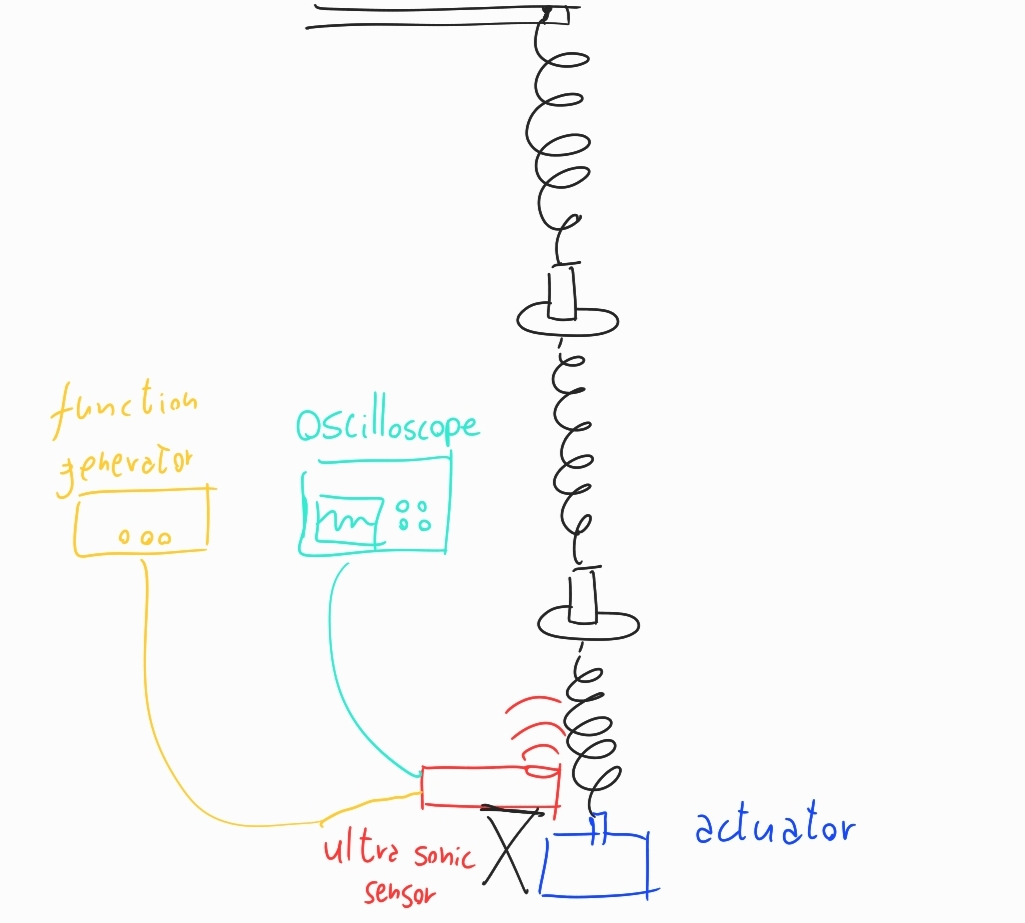
\includegraphics[width=0.48\textwidth]{Setup}
  \end{center}
  \label{img:setup}
  \caption{System setup}
\end{wrapfigure}
We call the two proper frequencies, phase and anti-phase frequency. If the system oscillates at the phase frequency, the two weights oscillate up and down, perfectly in sync. Instead if the system oscillates at the anti-phase frequency the two weights oscillate such that when one goes down, the other one goes up and vice versa. 

If we assume that the three springs are the same and the two masses are as well 
we derive the following formulas, where $k$ is the elastic coefficient of the springs, $m$ is the mass and the tilde is for the anti-phase frequency.
\begin{align}
    \nu_{th} &= \frac{1}{2\pi}   \sqrt{\frac{ k}{m}}
        \label{eq:nuth} \\
    \tilde \nu_{th} &= \frac{1}{2\pi}   \sqrt{\frac{3k}{m}}
        \label{eq:antinuth}
\end{align}
In this case we have that the ratio between the anti-phase and the phase frequency is $\sqrt 3$.

However when dealing with real masses and springs they most 
likely won't be equal. Without making the assumptions above 
the following formulas can be derived, where $k_i$ are the elastic coefficients of the springs, $M_i$ are the 2 masses, $m_i$ are the masses of the 3 springs and the tilde is for the anti-phase frequency.
\begin{align}
           \nu_{exp} &= \frac{1}{2\pi}   \sqrt{\frac{k_1+k_3}
           {M_1 + M_2 + \frac{1}{3} m_1 + m_2 + \frac{1}{3}m_3 }} 
           \label{eq:nuexp}  \\
    \tilde \nu_{exp} &= \frac{1}{2\pi}   \sqrt{\frac{k_1 +4k_2 +k_3}
           {M_1 + M_2 + \frac{1}{3} (m_1 + m_2 + m_3) }} 
           \label{eq:antinuexp} 
\end{align}
In this experiment we calculated these values and compared them with the frequencies we measured in various ways. 


%====================================================================================================================================
%====================================================================================================================================
%====================================================================================================================================
\section{First setup} \label{sec:setup1}
%devo dire static??
\begin{wraptable}{r}{4cm}
    \centering
    \begin{tabular}{|l|l|}
    \hline
         & massa \\ \hline
        1 & 0,0198 \\ \hline
        2 & 0,0999 \\ \hline
        3 & 0,1196 \\ \hline
        4 & 0,1393 \\ \hline
        5 & 0,1591 \\ \hline
    \end{tabular}
    \caption{Masses used for calculating k}
    \label{tab:regm}
\end{wraptable}
The first setup was to measure $k$, the elastic coefficient of the springs. 
%TODO  setup!!
To measure $k$ we used the following formula.
\begin{align}
    mg &= kx \\
    m  &= \frac{k}{g}x
\end{align}
%spiegare cos'è ogni singola variabile
The second formula shows the linear dependence between $m$ and $x$.

We attached one end of the spring to a metal support and we attached a tape measure to the same support so that they were both hanging vertically. Both were secured using adhesive tape. The tape measure could then be used to measure the position of the other end of the spring. We then attached different masses, one at a time, to the other end of the spring. When the masses are attached to the spring they begin to oscillate. We gradually slowed the mass down until it was still and then we measured its position on the tape measure beside it. 

We repeated this process for the 5 masses in table \ref{tab:regm} and by doing so we obtained different values for $x$ with the
corresponding values for $m$. We plotted these values to verify that
there was a linear relation between the two and we then made a linear
regression to find the coefficient $k/g$ with its corresponding
uncertainty. We then multiplied by $g$ both the value and its uncertainty to obtain $k$. 

The uncertainty we used in $x$ was 0,001 m.
%The uncertainty we used in $x$ was 0,002 m for "k_2" which was the first spring we studied, and 0,001 m for the other two. We used a higher uncertainty in the first spring because by studying the $\chi^2$ of the linear regression we realized we may have underestimated the uncertainty, as we were probably less precise since it was the first spring we studied. 

To test the fit of the data we did a $\chi^2$ test with $5-2 = 3$ degrees of freedom, and calculated the probability that the actual $\chi^2$ is higher than the value we obtained.

This same process was repeated for all 3 springs and the following values were obtained.
\begin{align}
    k_1 &= (20,3 \pm 0,4) \text{N/m} \quad \tilde \chi_1^2 = 0,09 \quad P_1 = 96\% \\
    k_2 &= (21,6 \pm 0,4) \text{N/m} \quad \tilde \chi_2^2 = 2,77 \quad P_2 =  5\% \\
    k_3 &= (20,7 \pm 0,4) \text{N/m} \quad \tilde \chi_3^2 = 0,28 \quad P_3 = 84\%
\end{align}
The second one has a high $\tilde \chi^2$, mainly due to the third mass. We realized this during the experiment, so we weighed the mass again and took the measurements again but we obtained the same values. We believe that either we underestimated the uncertainties or we made a mistake in the measurents, as even a difference of 0,001 m changes the $\tilde \chi^2$ significantly.

The three aren't compatible, as the second one is more than $2 \sigma$ away from the other two. 
%rivedi t test. NO! non t-test ma semplice gauss

%====================================================================================================================================
%====================================================================================================================================
%====================================================================================================================================
\section{Calculating $\bm \nu$ from k and m} \label{sec:nukm}

We then used equations \ref{eq:nuth} and \ref{eq:antinuth} from section \ref{sec:intro} to calculate $\nu_{th}$
and $\tilde \nu_{th}$. These formulas assume that all springs have
the same elastic coefficient, so we calculated a weighted average of
the different values of $k$ to use in these formulas. As can be seen from the more precise formula, the phase
frequency doesn't depend on the spring in the middle, and that's why we chose to put that spring in the middle. Also, because of this, the weighted average $k_{wav}$ was calculated only on spring 1 and 3.
Instead, for the frequency of anti-phase the weighted average 
$\tilde k_{wav}$ was calculated on all springs. We calculated the uncertainties in $k_{wav}$ and $\tilde k_{wav}$ with the formulas for the weighted average. 
\begin{align}
           k_{wav} &= (20,82 \pm 0,23) \text{N/m} \\
    \tilde k_{wav} &= (20,50 \pm 0,28) \text{N/m}
\end{align}
As $m$ we used $M_1=M_2=0,14210 \pm 0,00014$ kg, the sum of the mass of the cd and the weight. Its uncertainty was calculated as the root-sum-square of the uncertainties in the mass of the cd and of the weight.
To calculate the uncertainty in the frequencies we used the following formulas, where $\delta(\cdot)$ represents the uncertainty of the given variable.
\begin{equation} \label{eq:inc_nuth}
    \delta \nu_{th}
    = \frac{1}{2\pi} \frac{1}{2\sqrt{k/m}} \delta \left ( \frac{k}{m} \right )
    = \frac{1}{2\pi} \frac{1}{2\sqrt{k/m}}  \frac{k}{m} \sqrt{ \left ( \frac{ \delta k}{k}  \right ) ^2 +
           \left ( \frac{ \delta m}{m}  \right ) ^2}
\end{equation}
For the uncertainty in $\tilde \nu_{th}$ we used the same formula, with a factor of $\sqrt 3$. We obtained the following results
\begin{align}
           \nu_{th} &= (1,911 \pm 0,013) \text{Hz}\\
    \tilde \nu_{th} &= (3,337 \pm 0,019) \text{Hz}
\end{align}

Afterward, we used equations \ref{eq:nuexp} and \ref{eq:antinuexp} from section \ref{sec:intro} to calculate
$\nu_{exp}$ and $\tilde \nu_{exp}$. To calculate the uncertainty of the frequencies we first introduced the following variables.
\begin{align}
    M &= M_1 + M_2 + \frac{1}{3} m_1 + m_2 + \frac{1}{3}m_3\\
    K &= k_1 + k_3 \\
    \delta M &= \sqrt{
        ( \delta M_1)^2 + ( \delta M_2)^2 + 
        ( \delta \frac{m_1}{3} )^2 + ( \delta m_2)^2 + 
        ( \delta \frac{m_3}{3} )^2} \\
    \delta K &= \sqrt{
        ( \delta k_1)^2 + ( \delta k_3)^2 } \\
    \tilde M &= M_1 + M_2 + \frac{1}{3} (m_1 + m_2 + m_3) \\
    \tilde K &= k_1 +4k_2 +k_3 \\
    \delta \tilde M &= \sqrt{
        ( \delta M_1)^2 + ( \delta M_2)^2 + 
        ( \delta \frac{m_1}{3} )^2 + 
        ( \delta \frac{m_2}{3} )^2 +
        ( \delta \frac{m_3}{3} )^2} \\
    \delta \tilde K &= \sqrt{
        ( \delta k_1)^2 + ( \delta (4k_2))^2 + 
        ( \delta k_3)^2 } 
\end{align}
Formulas \ref{eq:nuexp} and \ref{eq:antinuexp} can now be written more simply as:
\begin{align}
    \nu_{exp} &= \frac{1}{2\pi}   \sqrt{\frac{ K}{M}} \\
    \tilde \nu_{exp} &= \frac{1}{2\pi}   \sqrt{
    \frac{\tilde K}{\tilde M}  }
\end{align}
And the uncertainty can be calculated with formulas analogous to \ref{eq:inc_nuth}


\begin{align}
\delta \nu_{exp} &= \frac{1}{2\pi} 
        \frac{1}{2\sqrt{K/M}}  \frac{K}{M} 
        \sqrt{ \left ( \frac{ \delta K}{K}  \right ) ^2 +
               \left ( \frac{ \delta M}{M}  \right ) ^2  } \\
    \delta \tilde \nu_{exp} &= \frac{1}{2\pi} 
        \frac{1}{2\sqrt{\tilde K/\tilde M}}  \frac{\tilde K}{\tilde M} 
        \sqrt{ \left ( \frac{ \delta \tilde K}{\tilde K}  \right ) ^2 +
               \left ( \frac{ \delta \tilde M}{\tilde M}  \right ) ^2  } 
\end{align}

With these calculations we obtained the following results.
\begin{align}
           \nu_{exp} &= (1,745 \pm 0,012) \text{Hz}\\
    \tilde \nu_{exp} &= (3,182 \pm 0,022) \text{Hz}
\end{align}

And for the ratio between the two we obtained the following result, which isn't compatible with $\sqrt 3$, the ratio between the theoretical frequencies. ??? di quanto?
\begin{equation}
    \tilde \nu_{exp} / \nu_{exp} = 1,823 \pm 0,013
\end{equation}

%====================================================================================================================================
%====================================================================================================================================
%====================================================================================================================================
\section{Second setup} \label{sec:setup2}
The second setup is the 2 mass, 3 spring system we want to examine. The springs and masses are setup as shown in the image \ref{img:setup}
In the middle we put the spring with the different elastic coefficient $k_2$, so that at least for the phase frequency the assumption that the springs have the same elastic coefficient is true. 
The spring on top is attached to a metal bar and the spring on the bottom is attached to the actuator. The actuator is connected to a function generator and to an oscilloscope to measure the frequency at which the it is oscillating. On a plate beside the actuator we placed the ultrasonic sensor which is connected to the computer program "Logger Pro". 

The transmitter in the sensor emits sound waves and the receiver sends an electric signal when the sound comes back. The device measures the time it takes for the sound to come back and it then divides by the speed of sound to obtain the position of the object that reflected the sound waves. So the sensor effectively gives us the position of the bottom mass at regular intervals that we set on Logger Pro. The program also calculates the FFT, so we have another way to read the frequency at which the system oscillates which we can compare to the value we read on the oscilloscope. 

%====================================================================================================================================
%====================================================================================================================================
%====================================================================================================================================
\section{Estimating $\bm \nu$ from the FFT of a generic motion}
The first way we measured the frequencies was by imposing a random motion on the masses and studying the FFT produced by Logger Pro. Without an external force, the system can only oscillate at its two proper frequencies, so by studying the FFT of the motion we should be able to identify the two proper frequencies. We did this process twice and obtained the following values. The uncertainty was estimated by calculating the width of the peak in the FFT for each frequency.
\begin{align}
           \nu_g^1 &= (1,729 \pm 0,015) \text{Hz} \quad        \nu_g^2 = (1,729 \pm 0,015) \text{Hz} \\
    \tilde \nu_g^1 &= (3,106 \pm 0,015) \text{Hz} \quad \tilde \nu_g^2 = (3,096 \pm 0,015) \text{Hz}
\end{align}
The two values for phase and the two for anti-phase were compatible so we calculated the two weighted averages and obtained the results below.
\begin{align}
           \nu_g &= (1,729 \pm 0,011) \text{Hz}\\
    \tilde \nu_g &= (3,101 \pm 0,011) \text{Hz}
\end{align}
We also calculated the ratio between the two and obtained $ \nu_g / \tilde \nu_g = 1,794 \pm 0,009$ which isn't compatible with $\sqrt 3$

%====================================================================================================================================
%====================================================================================================================================
%====================================================================================================================================
\section{Calculating $\bm \nu$ by measuring the period of oscillation}

The second way we measured the frequency was by making the two masses move in phase and then measuring the time it took to complete $n=10$ oscillations. This time was measured 5 times with the stopwatch and the same process was repeated for anti-phase. To make the masses move in phase, we manually lifted the two masses of approximately the same height and then let go. Instead, to make them move in anti-phase, we lifted one of the masses and lowered the other, by approximately the same height and then let go.

We then calculated the mean of the 5 values for phase and the 5 for anti phase. The results are shown below, along with the uncertainty of the mean. 
\begin{align}
           \nu_T &= (1,80 \pm 0,03) \text{Hz} \\
    \tilde \nu_T &= (2,96 \pm 0,13) \text{Hz}
\end{align}
We also calculated the ratio between the two and obtained $ \nu_T / \tilde \nu_T = 1,65 \pm 0,07$ which is compatible with $\sqrt 3$ within $1 \sigma$.
%includere medie e incertezze


%====================================================================================================================================
%====================================================================================================================================
%====================================================================================================================================
\section{Measuring $ \bm \nu $ from the resonance curve}
The final way we measured the frequencies was by studying the system with a driving external time-dependent sinusoidal force. By varying the driving frequencies we can reconstruct the resonance curve of the system, from which we can determine the proper frequency of the system, as it is the center of the curve. This is true in the approximation that $\Gamma^2 << \nu$ which can be assumed in this case. We repeated this process for both the phase frequency and the anti-phase frequency.


%====================================================================================================================================
%====================================================================================================================================
\subsection{Measuring $\bm \Gamma$}
The width of the resonance curve depends on $\Gamma$, the damping coefficient. The higher it, is the wider the resonance curve is. In order to reconstruct the curve, we want it to be as wide as possible, so we want $\Gamma$ to be as high as possible. This is why we attached disks to the masses, to increase friction and thus increase $\Gamma$ as well. Furthermore, $\Gamma$ depends on the masses used. Smaller masses will have a higher $\Gamma$, so we used a small mass. %perché non può esser minuscola??
To measure $\Gamma$ we would have had to impose the phase motion as explained above, activate the ultrasonic sensor from Logger Pro and wait for it to finish. After, we would have had to calculate the amplitude of motion near the beginning of the dataset??. To do this we had to find a maximum and an adjacent minimum of the position and calculate the semi-difference between the two. We call $A_i$ this amplitude and $t_i$ the average of the time measurement for the maximum and that of the minimum. We repeat the same process near the end of the dataset to obtain the values $A_f$ and $t_f$. $\Gamma$ can then be calculated as follows.
%\begin{align}
%    A(t) &= A_0 e^{-\frac{t}{2} \Gamma} \\
%    A_f / A_i &= e^{-\frac{t_f-t_i}{2} \Gamma} \\
%    \Gamma &= -2 \frac{ \ln(A_f / A_i) }{ t_f-t_i }
%\end{align}
\begin{equation}
    \Gamma = -2 \frac{ \ln(A_f / A_i) }{ t_f-t_i }
\end{equation}

We didn't do this process, but another group with similar masses and springs found $\Gamma = 0,023$ INCERTEZZA?? and $\tilde \Gamma = 0,031$
We measure $\Gamma$ because the FWHM of the resonance curve should be $\sqrt 3 \Gamma = 0,040$ for the phase frequency and $\sqrt 3 \tilde \Gamma = 0,054$ for the anti-phase frequency, so we later checked whether the FWHM of the curve was what we expected. VEDI CHE VALORI METTERE


%====================================================================================================================================
%====================================================================================================================================
\subsection{Resonance curve}
\begin{figure}
  \begin{center}
    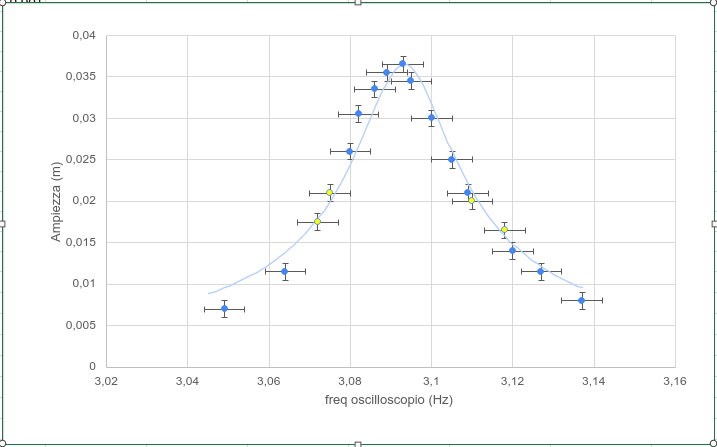
\includegraphics[width=0.8\textwidth]{lorentz_contro}
  \end{center}
  \label{img:res_contro}
  \caption{Resonance curve for anti-phase frequency}
\end{figure}
We started with the resonance curve for the phase frequency. We turned on the motor at a frequency close to the proper frequency we had previously measured with other methods. We started with this frequency to be sure that the oscillations of the system weren't too wide, as if this happened we saw the motion would start to become irregular, oscillating also from side to side. At this frequency, we regulated the amplitude of the function generator until we were satisfied with the oscillations of the system. We then started the ultrasonic sensor from Logger Pro and waited for the sampling to finish. We then checked the FFT from Logger Pro to be sure that the main frequency was the compatible to the value we had read on the oscilloscope. After, we measured the amplitude of the oscillations close to the end of the dataset as explained above. 

The same process, without changing the amplitude of the motor was repeated many times, slowly varying the driving frequency each time. 

The entire process was then repeated for the anti-phase frequency. The two resonance curves are shown. 
%grafici curve di risonanza
From this data we then measured all the parameters of the resonance curve: 
\begin{equation}
    a (\nu_d) = \frac{F/m}{  (2\pi)^2
                \sqrt{( \nu^2 - \nu_d^2 )^2 +
                \left ( \frac{\Gamma}{2\pi} \right )^2 \nu_d^2}}
\end{equation}  
Where $\nu$ is the proper frequency and $\nu_d$ is the driving frequency. To find $\Gamma$ we needed the FWHM, and to find the FWHM we needed the two frequencies that had an amplitude that was half the maximum. We assumed that the maximum was the highest amplitude we measured. To find those two points we interpolated between the points that were just above half maximum and just below. To propagate the uncertainties we used the standard formula with partial derivatives. The FWHM was then the difference between those two values. $\Gamma$ was then FWHM/$\sqrt 3$. And finally, we calculated $F/m$ from the maximum, which from the formula above with $\nu_d = \nu$ is given by: $F/m = 2\pi \nu a_{max} \Gamma$. 

We found the following values from the two curves:
\begin{align}
    \text{FWHM}        &= (0,034 \pm 0,006) \text{Hz}\\
    \text{FWHM}_{anti} &= (0,041 \pm 0,006) \text{Hz}\\
           \nu_R  &= (1,713 \pm 0,003) \text{Hz} \\
    \tilde \nu_R  &= (3,093 \pm 0,003) \text{Hz}
\end{align}
We also calculated the ratio between the two and obtained $ \nu_R / \tilde \nu_R = 1,806 \pm 0,004$ which isn't compatible with $\sqrt 3$.

%====================================================================================================================================
%====================================================================================================================================
%====================================================================================================================================
\section{Beats}
We then studied the beats phenomenon. This phenomenon is observed when the system oscillates at two close frequencies. In general, when a system oscillates at multiple frequencies, the overall oscillation is the sum of sinusoidal oscillations, each with it sown frequncy. When this is done with two close frequencies, the result of the sum takes a particular shape: the system oscillates at the average of the two frequencies $\nu_{av}$, but the amplitude of these oscillations isn't constant. The amplitude itself is also a sinusoidal function, with a frequency that is the semi-difference of the two frequencies $\nu_{beat}$. So if we study such a system and plot the position against?? time, we see a sinusoidal function with frequency $\nu_{av}$ enclosed in another sinusoidal function, with frequency $\nu_{beat}$. The image shows the result we obtained from frequencies $\nu_5$ and $\nu_6$ below.

\begin{wrapfigure}{r}{0.4\textwidth}
  \begin{center}
    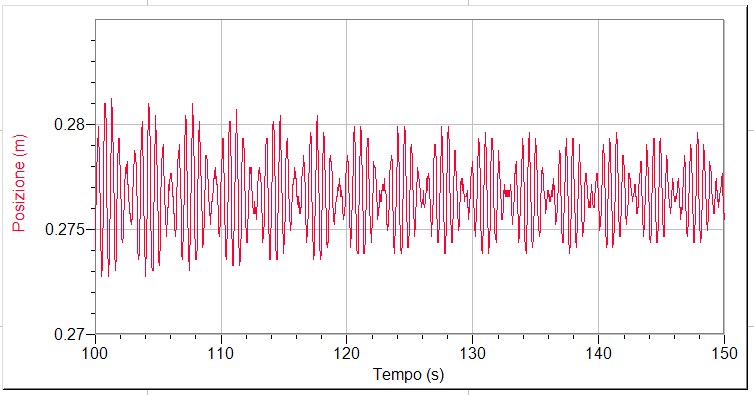
\includegraphics[width=0.48\textwidth]{battimenti_vicino_fase}
  \end{center}
  \label{img:beat}
  \caption{Beats from frequencies  $\nu_5$ and $\nu_6$}
\end{wrapfigure}

To have two frequencies with our setup, we started with a certain driving frequency and quickly changed it. This way the system continues to oscillate at the first frequency but als starts oscillationg at the second frequency. However, beacuse of friction the first frequency will die out ?? because the system loses energy and the driving force only gives energy ?? to the second frequency. Therefore the beats can be observed between when we change the driving frequency and when the first frequency disappears. 

To observe the phenomenon we activated the function generator at the anti-phase frequency and activated the ultrasonic sensor from Logger Pro with a sampling time of 500 s. After a few seconds, we quickly changed the driving frequency from the function generator. We then waited for the ultrasonic sensor to stop sampling. The frequencies, read from the oscilloscope and confirmed in Logger Pro are below.
\begin{equation}
    \nu_1 = ( 3,098 \pm 0,005) \text{Hz} \quad \nu_2 = ( 3,233 \pm 0,005) \text{Hz} 
\end{equation}
We then calculated the theoretical modulation frequency.
\begin{equation}
    \nu_{12} = \frac{|\nu_1 - \nu_2|}{2} = (0,068 \pm 0,004) \text{Hz}
\end{equation}
After, we measured the modulation period from the graph by finding three consecutive points in which the modulating amplitude is zero and taking the time difference between the first and the last one. We decided to take $0,2$ s as the time measurements, as we were certain that the exact point when the amplitude was zero was inside this range. For the uncertainty in the period we calculated the root-sum-square of the two uncertainties in the time measurements. We then calculated the experimental modulation frequency by taking the inverse of the period and obtained the following values. To calculate the uncertainty in this frequency we used the standard error propagation formula with partial derivatives.
\begin{align}
    T_{12} &= (15,0 \pm 0,3) \text{s} \\
    \nu_{12}^{exp} &= (0,0669 \pm 0,0013) \text{Hz} 
\end{align}
The measured and theoretical frequency are compatible within 0,2 $\sigma$.

We repeated this process starting with the phase frequency with the frequencies below and observed the same phenomenon. Theoretical and experimental modulation frequencies were then obtained as above:
\begin{align}
    \nu_{3} &= (1,719 \pm 0,005) \text{Hz} \\
    \nu_{4} &= (1,447 \pm 0,005) \text{Hz} \\
    \nu_{34} &= (0,136 \pm 0,004) \text{Hz} \\
    \nu_{34}^{exp} &= (0,131 \pm 0,005) \text{Hz} 
\end{align}
The two frequencies are compatible within 1 $\sigma$.

We then also repeated the process with the first frequency close to the phase frequency, to confirm that the phenomenon can be observed between any two frequencies, neither of the two has to be a proper frequency. First and second frequencies, along with theoretical and experimental modulation frequencies are shown below.
\begin{align}
    \nu_{5} &= (1,722 \pm 0,005) \text{Hz} \\
    \nu_{6} &= (2,021 \pm 0,005) \text{Hz} \\
    \nu_{56} &= (0,150 \pm 0,004) \text{Hz} \\
    \nu_{56}^{exp} &= (0,151 \pm 0,006) \text{Hz} 
\end{align}
The two frequencies are compatible within 0,2 $\sigma$.

\pagebreak
\section{Results}
We found the following values for the phase and anti-phase frequency. 
\begin{table}[h]
    \centering
    \begin{tabular}{|l|l|l|l|l|}
    \hline
         & ANTI-PHASE (Hz) &  & PHASE (Hz) &  \\ \hline
         & Values & Uncertainties & Values & Uncertainties \\ \hline
        Theoretical & 3,337 & 0,019 & 1,911 & 0,013 \\ \hline
        Experimental & 3,182 & 0,022 & 1,745 & 0,012 \\ \hline
        Generic motion & 3,101 & 0,015 & 1,729 & 0,015 \\ \hline
        Stopwatch & 2,96 & 0,13 & 1,80 & 0,03 \\ \hline
        Resonance curve & 3,093 & 0,003 & 1,713 & 0,003 \\ \hline
    \end{tabular}
    \caption{Frequency values}
\end{table}

From these values we made the following graphs to compare them
\begin{figure}[h]
  \begin{center}
    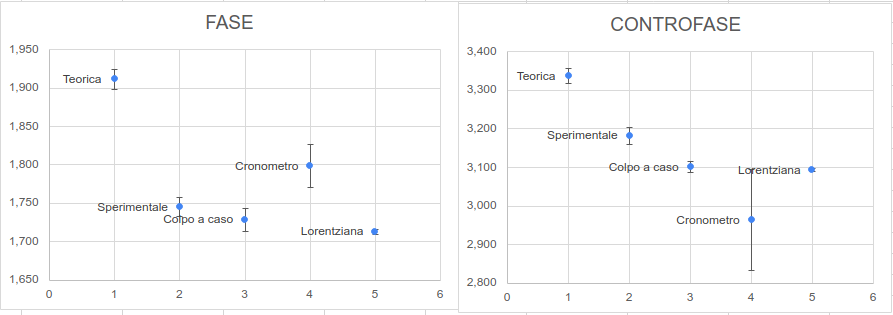
\includegraphics[width=\textwidth]{phase-anti}
  \end{center}
  \label{img:freq_comp}
  \caption{Beats from frequencies  $\nu_5$ and $\nu_6$}
\end{figure}

From the graphs we can see that the theoretical frequencies aren't compatible with any of other the other frequencies. While the experimental frequency is compatible with the stopwatch frequency, mainly because it has a large uncertainty. Instead its compatible with the generic motion frequency only for the phase. It's not compatible with the frequency from the resonance curve. Since all the measured frequencies are compatible, we believe  there must have a been a systematic error. We think that maybe the metal bar the top spring was attached to may have been oscillating, therefore altering the system and changing its proper frequencies. However we only thought of this after the experiment, so we weren't able to confirm it. 

Instead, regarding the beats, we were able to observe the phenomenon in all situations explained above and the measured frequency fit very well with the expected frequency.

\end{document}
